\documentclass{rapportECL}
\usepackage{lipsum}
\usepackage[table,xcdraw,svgnames]{xcolor}
\usepackage[tikz]{bclogo}

\title{Rapport ECL - Template} %Titre du fichier

\begin{document}

%----------- Informations du rapport ---------

\color{white}
\titre{Rapid prototyping of digital systems Labratory 1} %Titre du fichier .pdf
\UE{ELE8307} %Nom de la UE
\sujet{\LaTeX Approfondi} %Nom du sujet

\enseignant{Jean-Pierre \textsc{David}} %Nom de l'enseignant

\eleves{Hossein  \textsc{Askari} } %Nom des élèves

%----------- Initialisation -------------------
        
\fairemarges %Afficher les marges
\fairepagedegarde %Créer la page de garde
\tabledematieres %Créer la table de matières
\color{black}

%------------ Corps du rapport ----------------

\section{Lab1 Overview}


In this Lab, we got familiar with Altera (now Intel) FPGA design and synthesis tools. We learned how to use these tools to design, analyze, simulate and synthesize our design written in VHDL. The lab was divided into 3 parts:

\begin{itemize}
  \item Part1: First implementation of a PS2 keyboard module
  \item Part2: Fixing Synchronization problem
  \item Part3: Display result on 7-Segments
\end{itemize}

In the first part of the lab, we had to review the basic communication protocol used in PS2 keyboards. As it is illustrated in \ref{fig:ps2_wave}, the communication starts by bringing down the data line to zero. After that, the data will arrive in least significant bit order. After that, a parity bit  will be send and finally, the line will be driven to one to indicate end of communication.
\begin{figure}[h]
    \centering
    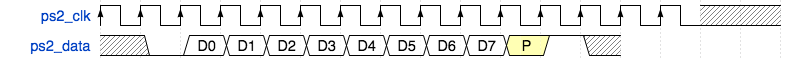
\includegraphics[width=15cm]{logos/ps2_wave.png}
    \caption{This is the waveform of a PS2 communication protocol. As it can be seen, the communication starts by bringing down the data line to zero. After that, the data will arrive in least significant bit order. After that, a parity bit  will be send and finally, the line will be driven to one to indicate end of communcation.}
    \label{fig:ps2_wave}
\end{figure}

In the following sections, we will use a pre-coded design to see this implementation in action.

\section{Lab1 Part1: Implementation de la premiere version du controleur clavier}
The objective of this part of the lab is to synthesis and implement a pre-coded PS2 communication protocol written in VHDL. We used \textbf{Quartus II} and \textbf{Cyclone II EP2C35F672C6} FPGA in this Lab. The following image shows a high level diagram of the implemented design. 

\begin{figure}[h]
    \centering
    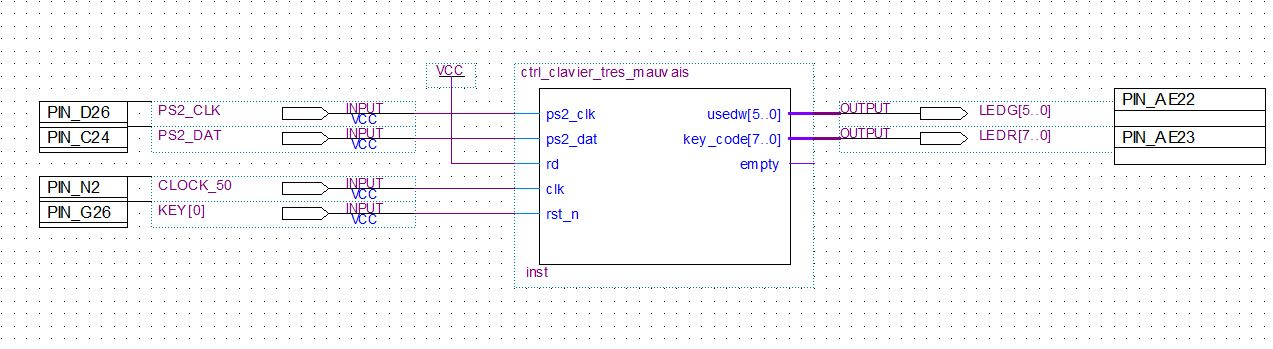
\includegraphics[width=15cm]{logos/part1_top.jpg}
    \caption{Top level design used in part1.}
    \label{fig:part1_top}
\end{figure}

We were asked to implement the design on FPGA and see if it operates correctly. We found out that it was not designed correctly. Figure \ref{fig:part1_mul_write_fifo} illustrates a gate-level simulation of the design. As it can be seen, the data seems to be extracted correctly. 

\begin{figure}[h]
    \centering
    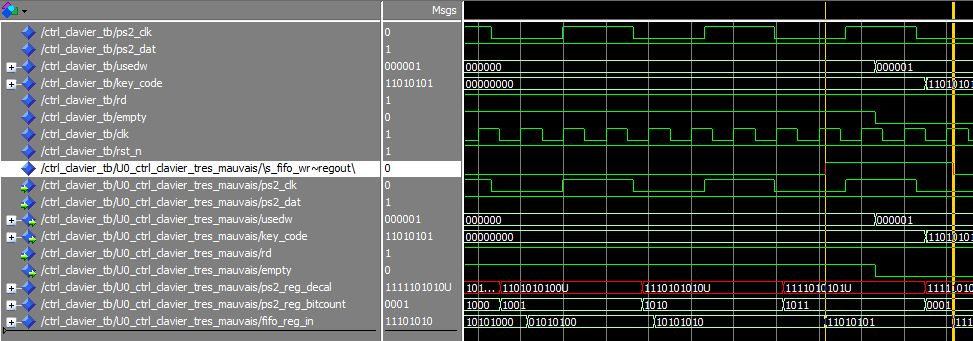
\includegraphics[width=15cm]{logos/top_part1.jpg}
    \caption{This waveform illustrates the operation of fifo write signal which results in writing multiple values to the fifo.}
    \label{fig:part1_mul_write_fifo}
\end{figure}

If you look closely, you will see that the fifo write signal is high for at least 3 clock cycles. This is because interaction with fifo is controled with a process that is synced with input 50MHz clock. On the other hand, the incoming data is synced with ps2\_clk. This will result in writing multiple values to the fifo. This has been shown in Figure \ref{fig:part1_mul_values_fifo}.

\begin{figure}[h]
    \centering
    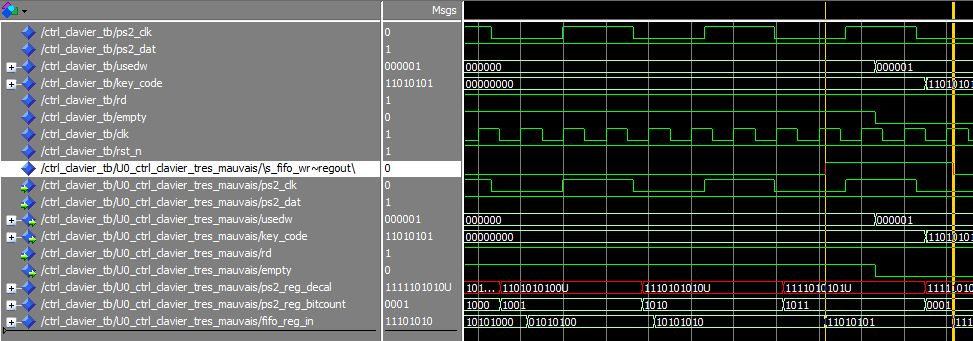
\includegraphics[width=15cm]{logos/top_part1.jpg}
    \caption{A closer look at the fifo write operation. By mistake, the transition values are being written into fifo. This is the result of using an un-synchronized processes to sample input data.}
    \label{fig:part1_mul_values_fifo}
\end{figure}
It is clearly shown that, by mistake, the transition values are being written into fifo. This is the result of using an un-synchronized processes to sample input data.

\begin{itemize}
    \item \textbf{Quel probleme observez-vous avec le registre fifo\_reg\_in}?\\ As it can be seen in the source code (ctrl\_clavier\_tres\_mauvais) , this register is being assigned a value that is updated in a separate process than the \textbf{fifo\_reg\_in}. This will result in writing wrong values to the fifo. This is a very bad practice in digital design.
    
    \item \textbf{Pouvez-vous l’expliquer} ?\\
    ps2\_reg\_decal is assigned to fifo\_reg\_in in \textbf{ACQ\_PROCESS\_FIFO} process, while, ps2\_reg\_decal is updated in \textbf{ACQ\_PROCESS\_PS2}. Having this alone is a bad practice. However, it gets even worst!. By looking closely to sensitivity list of these two process, we can see that we use two different clocks to assign the values. This will result in a horrible synchronization problem. 
    
    \item \textbf{Quel est le lien avec le registre ps2\_reg\_decal?}\\
    As it was explained previously, these two variables are in two different processes and they are being sampled with two different clocks. The best way is to design a synchronizer to sample the input data and clock from ps2 and use them in  \textbf{ACQ\_PROCESS\_PS2 process}.
\end{itemize}


\section{Lab1 Part2: Deuxième version du contrôleur PS/2}
In this part, we were asked to fix the problems with the previous design introduced in part 1. To better observe the issue, we were asked to use Quartus II Signal Tap software. Since the 50MHz clock would sample a lot of data in short amount of time, we down sampled the clock to 10MHz and then divided it to $\frac{1}{8}$ with a counter. This way we would observe the error much better. Figure \ref{fig:part2_top} illustrates the top level of the second part of this lab.

\begin{figure}[H]
    \centering
    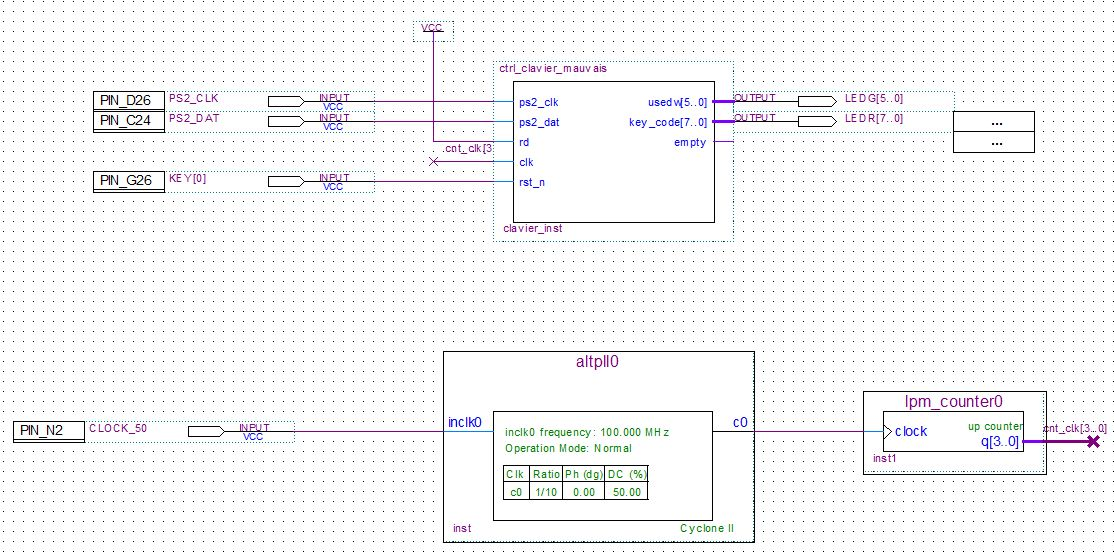
\includegraphics[width=15cm]{logos/part2_top.jpg}
    \caption{Top level design used in part2.}
    \label{fig:part2_top}
\end{figure}

We observed that although the design has changed from part1, but the synchronization error still remains the same. 



In this part of the lab we were asked to resolve this synchronization problem. There are several methods to resolve this issue:

\begin{itemize}
    \item Sample input on a much higher rate (at least, it should be more than Nyquist frequency of the input) which is not very common.
    \item Using a configurable PLL to lock on the input clock (very hard and not applicable to FPGA).
    \item Using Flip flop synchronizer.
    \item etc
\end{itemize}

Luckily, the input data rate is not very high and we should be able to synchronize on the input using a simple two flip flop synchronizer. Figure \ref{fig:2d_ff} clearly shows this method.

\begin{figure}[H]
    \centering
    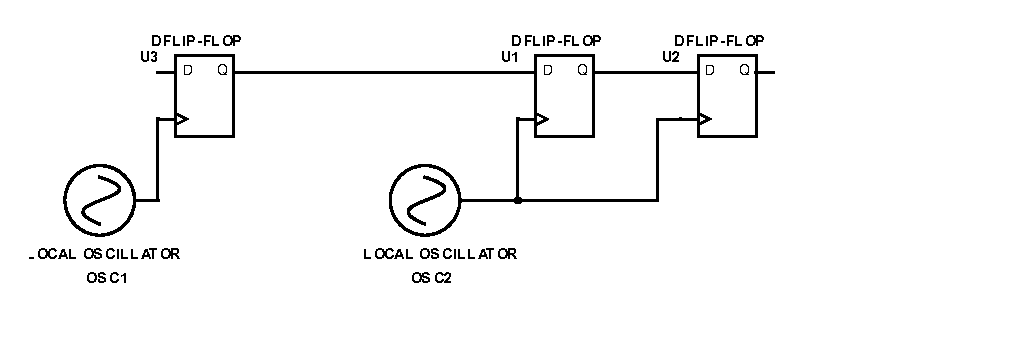
\includegraphics[width=15cm]{logos/2d_FF_sync.pdf}
    \caption{Two flip flop synchronizer method. This figure illustrates how to synchronize on the input data when it is being received on a different clock domain. }
    \label{fig:2d_ff}
\end{figure}

Figure \ref{fig:2d_ff} illustrates how to synchronize on the input data when it is being received on a different clock domain. There is probability that while sampling the input U1-D by flip flop U1 in OSC2 clock domain, output U1-Q may go into a meta-stable state. But during the one clock cycle period of OSC2 clock, output U1-Q may settle to some stable value. Output of flop U2 can go to meta-stable if U1 does not settle to stable value during one clock cycle, but probability for U2 to be meta-stable for a complete destination clock cycle is close to zero. This method will help to synchronize on input when the input data rate is low. For higher data rates, multiple flip-flop stages can help for synchronization.

\begin{bclogo}[logo=\bcinfo, couleurBarre=orange, noborder=true, couleur=white]{Warning!}
This method has a draw back. Adding more flip-flop stages can cause slack delay on the data path line. For higher data rates it is advised to use different methods of synchronization.
\end{bclogo}



\section{Lab1 Part3: Utilisation de modules IP}
In this part, we were asked to use IP modules to display the received data on the available 7-segments. We were also asked to design a circuit that would convert an 8-bit input binary to a 3-digit Binary Coded Decimal (BCD) value. This way, we would be able to use three 7-segments to display values between 0 to 255.\\
There are different methods to achieve this goal. One could use 3 stage of division to extract hundreds, tens and ones of the input data. We decided to use a fully combinational circuit. We also didn't bother to use a division IP block. The following table shows a common way to convert a binary input to a BCD value.

% Please add the following required packages to your document preamble:
% \usepackage[table,xcdraw]{xcolor}
% If you use beamer only pass "xcolor=table" option, i.e. \documentclass[xcolor=table]{beamer}
\begin{table}[H]
\centering
\captionof{table}{Example of Binary to BCD algorithm} \label{tab:title2} 

\begin{tabular}{|l|l|l|l|l|}
\hline
100's                    & 10's                        & 1's                         & Binary                  & Operation               \\ \hline
                         &                             &                             & 1001 0101               &                         \\ \hline
                         &                             & 1                           & 001  0101               & SHL \#1                 \\ \hline
                         &                             & 10                          & 01 0101                 & SHL \#2                 \\ \hline
                         &                             & 100                         & 1 0101                  & SHL \#3                 \\ \hline
                         &                             & 1001                        & 0101                    & SHL \#4                 \\ \hline
                         &                             & 1100                        &                         & ADD 3                   \\ \hline
                         & 1                           & 1000                        & 101                     & SHL \#5                 \\ \hline
                         &                             & 1011                        &                         & ADD3                    \\ \hline
                         & 11                          & 0111                        & 01                      & SHL \#6                 \\ \hline
                         &                             & 1010                        &                         & ADD 3                   \\ \hline
                         & 111                         & 0100                        & 1                       & SHL \#7                 \\ \hline
                         & 1010                        &                             &                         & ADD 3                   \\ \hline
{1} & { 0100} & {1001} & & \\ \hline\hline
1                        & 4                           & 9                           &                         & Final Value             \\ \hline
\end{tabular}
\end{table}

We wrote a VHDL code to convert the input binary value to a 3-digit BCD value. The final top level schematic is illustrated in Figure \ref{fig:part3_top}.

\begin{figure}[H]
    \centering
    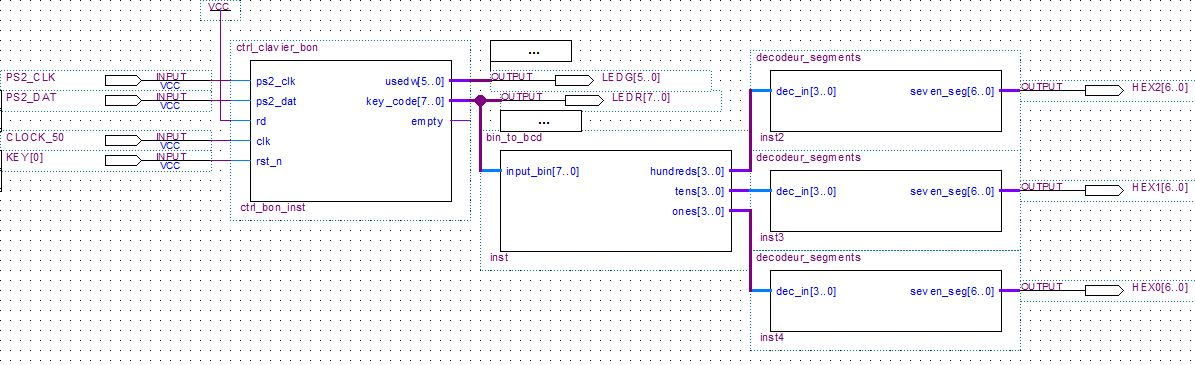
\includegraphics[width=15cm]{logos/part3_top.jpg}}
    \caption{ This is the schematic view of the circuit designed for part3 of the lab. }
    \label{fig:part3_top}
\end{figure}

Finally, we used the provided \textbf{decodeur7segments.vhd} to display the values on the seven segments.
\end{document}
